% =====================================================================
%  Física de los mercados: cuatro ideas
%  Compilar con pdfLaTeX + BibTeX (en Overleaf funciona tal cual).
% =====================================================================
\documentclass[11pt,a4paper]{article}

\usepackage[T1]{fontenc}
\usepackage[utf8]{inputenc}
\IfFileExists{spanish.ldf}%
  {\usepackage[spanish,es-noshorthands,es-tabla,es-nodecimaldot]{babel}}%
  {\usepackage[provide=*,spanish]{babel}}
\usepackage{mathpazo}
\linespread{1.08}
\usepackage{microtype}
\usepackage[a4paper,top=2.7cm,bottom=2.7cm,left=2.9cm,right=2.9cm]{geometry}
\usepackage{amsmath,amssymb}
\usepackage{graphicx}
\graphicspath{{figuras/}}
\usepackage{booktabs,array}
\usepackage{xcolor}
\usepackage[font=small,labelfont=bf,labelsep=period]{caption}
\usepackage{enumitem}
\setlist{itemsep=2pt,topsep=4pt}
\usepackage[numbers,sort&compress]{natbib}
\usepackage[hidelinks]{hyperref}
\usepackage[spanish,noabbrev]{cleveref}
\crefname{section}{sección}{secciones}
\Crefname{section}{Sección}{Secciones}
\setcounter{tocdepth}{1}
\usepackage{titlesec}
\titleformat{\section}{\Large\bfseries}{\thesection.}{0.6em}{}
\titleformat{\subsection}{\large\bfseries}{\thesubsection}{0.6em}{}
\setlength{\parskip}{0.35em}
\setlength{\emergencystretch}{2em}

\newcommand{\E}{\mathbb{E}}
\newcommand{\dd}{\mathrm{d}}
\newcommand{\autor}{Tu Nombre}   % <-- pon aquí tu nombre

\title{\textbf{Física de los mercados: cuatro ideas}\\[0.4em]
\large Mecánica estadística y materia condensada aplicadas a los precios}
\author{\autor}
\date{Octubre de 2026}

\begin{document}
\maketitle

\begin{abstract}
\noindent Este documento cuenta cuatro ideas de la física estadística que ayudan a entender cómo se
mueven los precios en bolsa: el movimiento browniano, la temperatura, una partícula atada a un muelle y el
modelo de Ising. Cada idea se presenta primero en su versión física, después se traduce a la economía y,
por último, se pone a prueba con datos reales (Google entre 2004 y 2008, y los índices S\&P~500 y Nasdaq
entre 1990 y 2022). No hace falta saber nada de finanzas: los términos económicos se explican cuando
aparecen. Cada sección tiene un programa corto en Python que reproduce sus figuras y sus números.
\end{abstract}

\tableofcontents

% =====================================================================
\section{Introducción: un mercado visto como un gas}
% =====================================================================

\subsection{Lo mínimo de economía que necesitamos}

Una \emph{acción} es un trozo pequeño de una empresa. Quien la tiene es dueño de una parte de esa empresa
y puede venderla cuando quiera en la bolsa. La bolsa funciona como una subasta que no se detiene nunca:
unos quieren comprar, otros quieren vender, y el \emph{precio} es simplemente el último al que se han
puesto de acuerdo un comprador y un vendedor. Si en un momento hay más gente con ganas de comprar que de
vender, los compradores tienen que ofrecer un poco más para conseguir acciones y el precio sube. Si hay más
vendedores, baja. No hace falta saber más para seguir este texto: el precio se mueve porque se mueve el
equilibrio entre compradores y vendedores.

Para estudiar cómo se mueve el precio no se mira el precio en sí, sino su cambio de un día a otro. Lo
llamamos \emph{retorno}, y lo definimos con un logaritmo:
\begin{equation}
r_t=\ln\frac{P_t}{P_{t-1}} ,
\end{equation}
donde $P_t$ es el precio al cierre del día $t$. Si el precio pasa de 100 a 102, $r=\ln1.02=0.0198$, casi
exactamente un 2\%. Para cambios pequeños el retorno es, en la práctica, el cambio porcentual. El
logaritmo tiene una ventaja que usaremos todo el rato: los retornos de días consecutivos se \emph{suman}.
El retorno de una semana es la suma de los cinco retornos diarios, igual que la posición de un caminante es
la suma de sus pasos.

La segunda palabra que necesitamos es \emph{volatilidad}. Es la desviación típica $\sigma$ de los
retornos: cuánto se mueve el precio en un día típico, sea hacia arriba o hacia abajo. Para Google en
2004--2008, $\sigma=2.36\%$ diario. Una acción con $\sigma=1\%$ es tranquila; una con $\sigma=4\%$ es muy
agitada. Para un inversor, la volatilidad es la medida más directa del \emph{riesgo}.

Por último, un \emph{índice bursátil} es una media ponderada de los precios de muchas empresas. El
S\&P~500 resume las 500 mayores empresas de Estados Unidos; el Nasdaq está dominado por empresas
tecnológicas. Funcionan como un termómetro del mercado en su conjunto.

\subsection{Por qué la física tiene algo que decir}

En un gas hay del orden de $10^{23}$ moléculas. Nadie intenta seguir a cada una; la mecánica estadística
renuncia a eso y busca leyes para las magnitudes colectivas (presión, temperatura) que surgen de muchos
movimientos individuales desordenados. Un mercado es parecido: millones de personas y programas que
compran y venden por razones distintas, la mayoría desconocidas. No sabemos por qué compra cada uno, pero
podemos preguntarnos qué regularidades estadísticas produce el conjunto. Esa es la idea de la
\emph{econofísica} \cite{mantegna2000,bouchaud2003}.

El paralelismo no es sólo una metáfora: la primera teoría matemática del movimiento browniano no la
escribió Einstein en 1905 \cite{einstein1905}, sino Louis Bachelier en 1900, en una tesis doctoral sobre
los precios de la bolsa de París \cite{bachelier1900}.

\subsection{Los datos y el plan}

Usamos dos conjuntos de datos reales, que vienen incluidos con la librería \texttt{matplotlib} de Python
(no hace falta descargar nada):
\begin{itemize}
\item el precio diario de cierre de Google desde su salida a bolsa (agosto de 2004) hasta octubre de
2008: 1047 días, que dan 1046 retornos. Incluye una época de fuerte crecimiento y el inicio de la crisis
financiera de 2008;
\item el valor mensual del S\&P~500 y del Nasdaq entre 1990 y 2022: 391 meses, que incluyen la burbuja
tecnológica de 2000.
\end{itemize}

El documento tiene cuatro partes, una por idea física (\cref{tab:plan}). Cada una sigue el mismo orden:
primero la física, después la traducción económica y al final los datos.

\begin{table}[ht]
\centering\small
\caption{Las cuatro ideas del documento.}
\label{tab:plan}
\begin{tabular}{@{}l>{\raggedright\arraybackslash}p{3.6cm}>{\raggedright\arraybackslash}p{5.0cm}>{\raggedright\arraybackslash}p{3.9cm}@{}}
\toprule
& Idea física & Fenómeno económico & Programa \\
\midrule
\S\ref{sec:paseo} & movimiento browniano, difusión & el precio es impredecible; el riesgo crece como $\sqrt t$ & \texttt{01\_paseo\_aleatorio.py}\\
\S\ref{sec:temp} & temperatura de un baño térmico & épocas tranquilas y agitadas; caídas extremas & \texttt{02\_temperatura.py}\\
\S\ref{sec:muelle} & partícula en un muelle (Langevin) & diferencias de precio que vuelven a su nivel & \texttt{03\_muelle.py}\\
\S\ref{sec:ising} & modelo de Ising & imitación, burbujas y crashes & \texttt{04\_ising.py}\\
\bottomrule
\end{tabular}
\end{table}

% =====================================================================
\section{El precio como partícula browniana}
\label{sec:paseo}
% =====================================================================

\subsection{La física: un caminante sin memoria}

Una partícula de polen en agua recibe choques de las moléculas que la rodean. Cada choque la empuja un poco
en una dirección al azar, y un choque no tiene nada que ver con el anterior. Si llamamos $x_t$ a su posición
después de $t$ intervalos de tiempo,
\begin{equation}
x_t=x_0+\xi_1+\xi_2+\dots+\xi_t ,
\end{equation}
con pasos $\xi_k$ independientes, de media $\mu$ y varianza $\sigma^2$. Es el paseo aleatorio.

La propiedad central sale en una línea: las varianzas de variables independientes se suman, así que
\begin{equation}
\langle(x_t-x_0-\mu t)^2\rangle=\sigma^2\,t .
\label{eq:difusion}
\end{equation}
El desplazamiento cuadrático medio crece \emph{linealmente} con el tiempo; el desplazamiento típico, como
$\sqrt t$. Esto es la difusión. En el límite continuo, la densidad de probabilidad de la posición cumple la
ecuación de difusión,
\begin{equation}
\frac{\partial p}{\partial t}=D\,\frac{\partial^2p}{\partial x^2},\qquad D=\frac{\sigma^2}{2},
\end{equation}
cuya solución, partiendo de un punto, es una gaussiana que se ensancha como $\sqrt{2Dt}$. Además, por el
teorema central del límite, la suma de muchos pasos es gaussiana aunque cada paso no lo sea.

\subsection{La traducción económica}

Tomemos $x_t=\ln P_t$, el logaritmo del precio. Entonces cada paso es un retorno, $\xi_t=r_t$, y el modelo
de Bachelier dice que los retornos son independientes entre sí.

¿Por qué iban a serlo? El argumento es económico y muy sencillo. Supón que todo el mundo supiera que
mañana Google va a subir un 3\%. Entonces todos querrían comprar hoy, a cualquier precio por debajo del de
mañana, y esa avalancha de compradores subiría el precio \emph{hoy}. La subida prevista desaparece en el
momento en que se prevé. Si la información pública sobre el futuro ya está incorporada en el precio de
hoy, lo único que puede mover el precio mañana es información nueva, y la información nueva, por
definición, no se puede predecir. Esto se conoce como \emph{hipótesis de los mercados eficientes}
\cite{fama1970}. No tiene por qué ser exacta, pero da una razón para esperar que los retornos se parezcan
a los choques al azar del polen.

\begin{table}[ht]
\centering\small
\caption{Diccionario de esta sección.}
\begin{tabular}{@{}ll@{}}
\toprule
Física & Mercado \\
\midrule
posición $x_t$ de la partícula & logaritmo del precio, $\ln P_t$\\
paso $\xi_t$ & retorno diario $r_t$\\
choques de las moléculas & llegada de noticias y de órdenes de compra y venta\\
deriva $\mu$ & tendencia media del precio\\
coeficiente de difusión $D=\sigma^2/2$ & volatilidad al cuadrado (sobre dos)\\
\bottomrule
\end{tabular}
\end{table}

\Cref{fig:paseos} es un pequeño juego. Las cuatro curvas empiezan en 100 dólares. Tres son paseos
aleatorios simulados con la media y la volatilidad de Google; una es el precio real de Google. ¿Cuál es? La
respuesta está en el pie de la figura, pero merece la pena intentarlo antes de mirar. Lo normal es no
acertar con seguridad: a simple vista, el precio real es indistinguible de un paseo aleatorio.

\begin{figure}[ht]
\centering
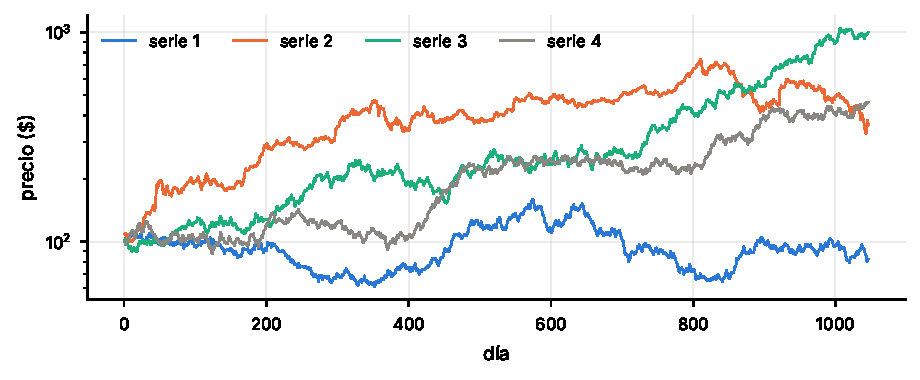
\includegraphics[width=0.95\textwidth]{fig1_paseos.pdf}
\caption{Tres paseos aleatorios con la misma media y volatilidad que Google, y el precio real de Google
(agosto de 2004 a octubre de 2008), en escala logarítmica. El real es la serie 2.}
\label{fig:paseos}
\end{figure}

\subsection{Consecuencia práctica: el riesgo crece como la raíz del tiempo}

La ecuación \eqref{eq:difusion} tiene una consecuencia económica inmediata. Si la volatilidad diaria es
$\sigma$, la de un periodo de $t$ días es $\sigma\sqrt t$, no $\sigma\,t$. Con los números de Google:
\begin{itemize}
\item un día: $2.36\%$;
\item un mes (unos 21 días de mercado): $2.36\%\times\sqrt{21}=10.8\%$;
\item un año (252 días de mercado): $2.36\%\times\sqrt{252}=37.5\%$.
\end{itemize}
Si el riesgo creciera linealmente, el anual sería del $595\%$. Esta regla de la raíz cuadrada es la que
usan todos los bancos para pasar de un horizonte a otro.

Hay una segunda consecuencia, más sutil. La deriva (la tendencia) crece como $\mu t$, pero el ruido crece
sólo como $\sigma\sqrt t$. Su cociente, una especie de relación señal/ruido, crece como $\sqrt t$. En Google,
$\mu=0.12\%$ diario: en un día la tendencia es veinte veces más pequeña que el ruido ($0.12$ frente a
$2.36$) y resulta invisible; en un año la tendencia acumulada ($31\%$) ya es comparable al ruido ($37\%$).
Por eso invertir a largo plazo y especular a corto plazo son actividades muy distintas: a corto plazo
domina por completo el azar.

\subsection{¿Lo cumplen los datos?}

Comprobamos con los 1046 retornos de Google las dos predicciones del modelo: que no hay memoria y que la
varianza crece linealmente (\cref{fig:difusion}).

\paragraph{Memoria.} La autocorrelación $C(\tau)$ mide cuánto se parece el retorno de hoy al de hace
$\tau$ días: vale 1 si son iguales, $-1$ si son opuestos y 0 si no tienen relación. Para un paseo
aleatorio, $C(\tau)=0$; con datos finitos sale un valor pequeño que fluctúa dentro de una banda de anchura
$\pm1.96/\sqrt n=\pm0.061$ el 95\% de las veces. Medimos $C(1)=0.024$, dentro de la banda. De los 20
primeros retardos, 2 salen ligeramente fuera, lo que se espera por azar (el 5\% de 20 es 1, con
fluctuaciones). El retorno de hoy no dice nada útil sobre el de mañana.

\paragraph{Difusión.} Calculamos la varianza de los retornos sumados a $k$ días, para $k$ entre 1 y 60.
En escala doble logarítmica, una ley $\propto k$ es una recta de pendiente 1. Medimos una pendiente de
$1.10$: muy cerca. El pequeño exceso viene de que 2004--2008 fue una época de tendencias largas, que hacen
que los retornos de muchos días se acumulen algo más de lo que lo haría un paseo puro.

\begin{figure}[ht]
\centering
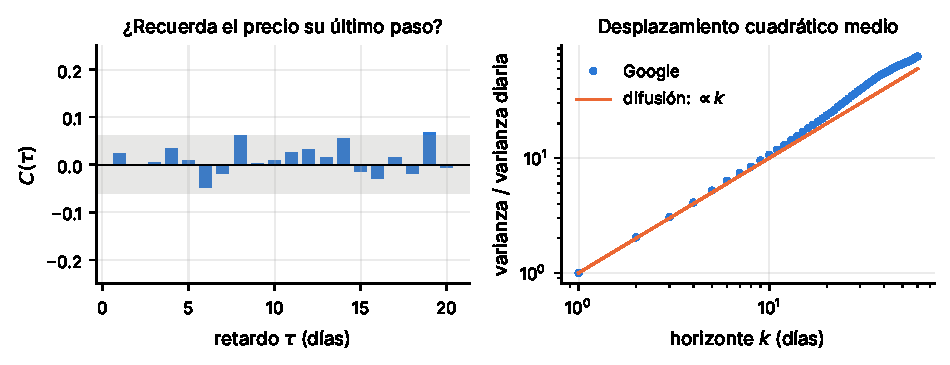
\includegraphics[width=\textwidth]{fig1_difusion.pdf}
\caption{Izquierda: autocorrelación de los retornos diarios de Google; la banda gris es la zona
compatible con ausencia de memoria. Derecha: varianza de los retornos a $k$ días, dividida por la
diaria, frente a la recta de difusión.}
\label{fig:difusion}
\end{figure}

\subsection{Dónde falla: los días extremos}

La tercera predicción del modelo es que, al ser sumas de muchos choques, los retornos diarios deberían ser
gaussianos. Aquí el modelo falla, y falla precisamente donde más importa. Midamos cada retorno en
unidades de desviación típica, $z=(r-\mu)/\sigma$, y contemos los días que superan un umbral:

\begin{table}[ht]
\centering\small
\caption{Días de Google con un movimiento mayor que el umbral (en cualquier sentido), observados y
esperados si los retornos fueran gaussianos.}
\label{tab:extremos}
\begin{tabular}{@{}lcc@{}}
\toprule
Umbral & Observados & Esperados (gaussiana)\\
\midrule
$|z|>3$ & 16 & 2.8\\
$|z|>4$ & 6 & 0.07\\
$|z|>5$ & 4 & 0.0006\\
\bottomrule
\end{tabular}
\end{table}

Un día de más de 5 desviaciones típicas debería ocurrir, si los retornos fueran gaussianos, una vez cada
6900 años. En estos cuatro años ocurrió cuatro veces. La \cref{fig:colas} lo muestra: en escala
logarítmica la gaussiana es una parábola que cae muy deprisa, mientras que los datos tienen
\emph{colas gruesas}. Una forma de resumirlo es la curtosis en exceso, que vale 0 para una gaussiana y
$7.6$ para Google. Mandelbrot ya lo señaló en 1963 con los precios del algodón \cite{mandelbrot1963}, y es
una de las regularidades más universales de los mercados \cite{cont2001}.

\begin{figure}[ht]
\centering
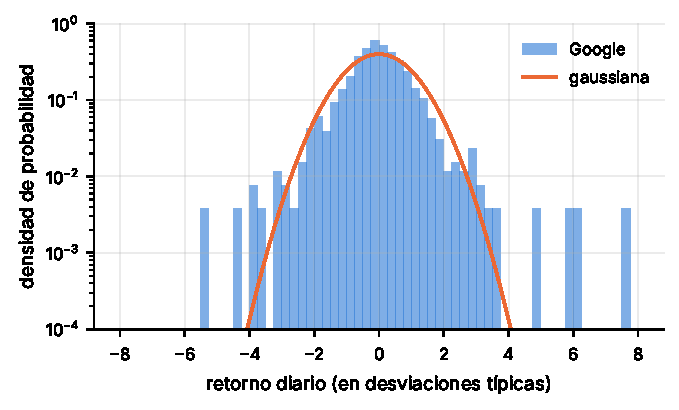
\includegraphics[width=0.7\textwidth]{fig1_colas.pdf}
\caption{Histograma de los retornos diarios de Google en desviaciones típicas, frente a la gaussiana, en
escala logarítmica. Las barras aisladas a la izquierda y a la derecha son días que una gaussiana no
produciría nunca.}
\label{fig:colas}
\end{figure}

¿Qué hipótesis del paseo aleatorio se rompe? El teorema central del límite necesita pasos independientes
e \emph{idénticamente distribuidos}. La siguiente sección muestra que la segunda condición es la que falla:
no todos los días son iguales, porque la ``temperatura'' del mercado cambia.

% =====================================================================
\section{La volatilidad como temperatura}
\label{sec:temp}
% =====================================================================

\subsection{La física: una partícula en un baño térmico}

En un gas en equilibrio a temperatura $T$, cada componente de la velocidad de una molécula sigue la
distribución de Maxwell--Boltzmann, que es una gaussiana de varianza
\begin{equation}
\langle v^2\rangle=\frac{k_BT}{m}.
\end{equation}
La temperatura es literalmente la anchura de la distribución de velocidades. Cuanto más caliente está el
gas, más deprisa se mueven las moléculas en promedio, en cualquier dirección.

Ahora la idea clave. Si la temperatura \emph{no es la misma todo el tiempo}, por ejemplo porque el baño se
calienta y se enfría lentamente, y medimos velocidades durante mucho rato, lo que obtenemos es una
\emph{mezcla} de gaussianas de distinta anchura. Y una mezcla de gaussianas no es una gaussiana: tiene
más peso en el centro (los momentos fríos) y mucho más peso en las colas (los momentos calientes). Esta
idea tiene nombre en física estadística: \emph{superestadística} \cite{beck2003}.

\subsection{La traducción económica}

El retorno de un día hace el papel de la velocidad de la molécula, y la volatilidad, el de la
temperatura: $\sigma^2\leftrightarrow k_BT$. Un mercado ``caliente'' es uno en el que los precios se
mueven mucho cada día, en cualquier dirección. Ocurre cuando hay incertidumbre: una crisis, una
guerra, unas elecciones, o simplemente cuando una empresa está a punto de publicar sus resultados. Un
mercado ``frío'' es uno tranquilo.

\begin{table}[ht]
\centering\small
\caption{Diccionario de esta sección.}
\begin{tabular}{@{}ll@{}}
\toprule
Física & Mercado \\
\midrule
velocidad de una molécula & retorno de un día\\
temperatura, $k_BT/m$ & volatilidad al cuadrado, $\sigma^2$\\
baño que se calienta y se enfría & épocas tranquilas y épocas de crisis\\
mezcla de temperaturas & colas gruesas\\
tiempo de relajación de la temperatura & cuánto dura una época agitada\\
\bottomrule
\end{tabular}
\end{table}

\subsection{Un termómetro para el mercado}

La forma más sencilla de medir la temperatura de cada día es calcular la desviación típica de los
retornos de los 20 días anteriores (aproximadamente un mes). \Cref{fig:termometro} muestra el resultado
para Google, expresado en volatilidad anual. La temperatura no es constante en absoluto: va de un $12\%$
anual en la calma de 2007 a un $86\%$ en octubre de 2008. Y los días agitados no aparecen sueltos, sino
en rachas. Es el \emph{agrupamiento de volatilidad}.

\begin{figure}[ht]
\centering
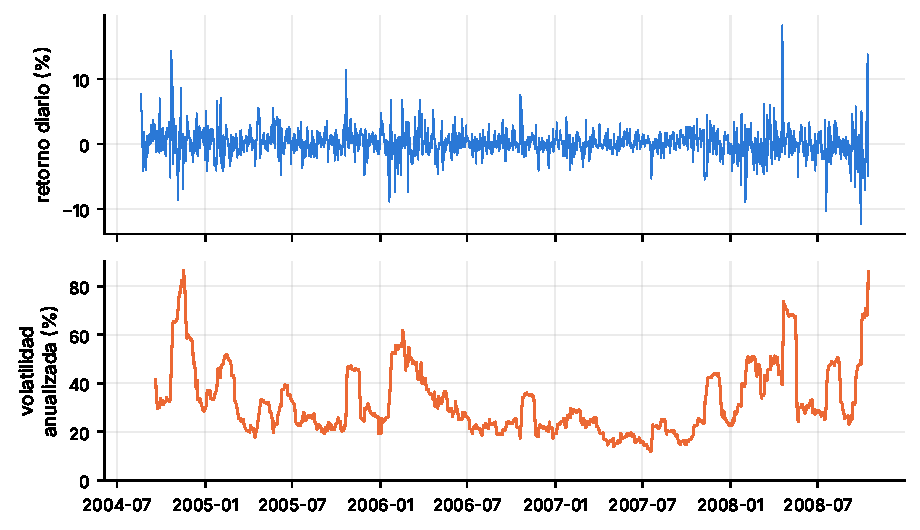
\includegraphics[width=0.95\textwidth]{fig2_termometro.pdf}
\caption{Arriba: retornos diarios de Google. Abajo: su ``temperatura'', medida como la volatilidad de los
20 días anteriores (anualizada).}
\label{fig:termometro}
\end{figure}

\subsection{El signo no tiene memoria, el tamaño sí}

En la sección anterior vimos que el retorno de hoy no predice el de mañana. Pero si en lugar de $r_t$
miramos su tamaño $|r_t|$, sin signo, la historia cambia (\cref{fig:memoria}). La autocorrelación de
$|r_t|$ vale $0.148$ a un día y se mantiene positiva durante semanas: su media en los primeros 20 días es
$0.093$, frente a $0.011$ para $r_t$. Un día agitado suele ir seguido de otro día agitado, aunque no
sepamos si será de subida o de bajada.

\begin{figure}[ht]
\centering
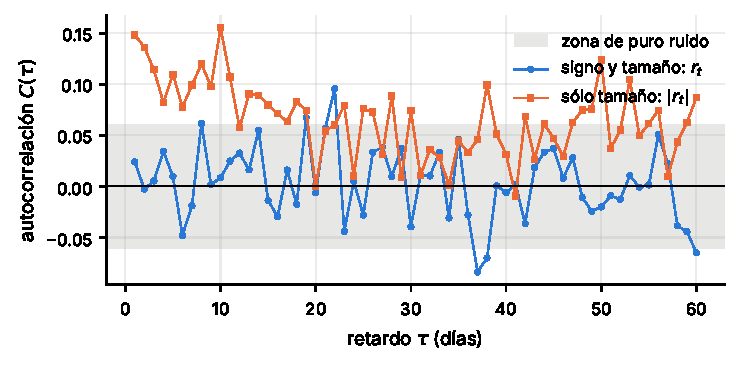
\includegraphics[width=0.75\textwidth]{fig2_memoria.pdf}
\caption{Autocorrelación del retorno $r_t$ (azul) y de su tamaño $|r_t|$ (naranja) para retardos de 1 a 60
días. La banda gris es la zona compatible con ruido puro.}
\label{fig:memoria}
\end{figure}

En lenguaje físico: hay una \emph{separación de escalas de tiempo}. La ``velocidad'' (el retorno) se
descorrelaciona en un día, pero la ``temperatura'' (la volatilidad) es una variable lenta que cambia en
semanas o meses. Es la misma situación que una partícula browniana en un baño que se calienta despacio.

\subsection{Un ejemplo de juguete: dos temperaturas bastan}

Supongamos el mercado más sencillo posible con dos temperaturas: el $80\%$ de los días son fríos, con
$\sigma=1.5\%$, y el $20\%$ son calientes, con $\sigma=4\%$. Cada día, por separado, es gaussiano. Hagamos
las cuentas:
\begin{itemize}
\item La varianza total es la media de las varianzas:
$0.8\times1.5^2+0.2\times4^2=5$, es decir, $\sigma_{\text{total}}=2.24\%$ (muy parecida a la de Google).
\item El cuarto momento de cada gaussiana es $3\sigma^4$, así que el de la mezcla es
$3(0.8\times1.5^4+0.2\times4^4)=165.75$, y la curtosis en exceso, $165.75/5^2-3=3.6$. Una sola gaussiana
tendría 0.
\item La probabilidad de una caída de más del $8\%$ en un día es $0.46\%$ con la mezcla, y $0.017\%$ con una
gaussiana de la misma volatilidad total. \emph{Veintiséis veces más}.
\end{itemize}
La \cref{fig:mezcla} lo muestra en escala logarítmica. La mezcla (negro) coincide con la gaussiana en el
centro, pero en las colas está dominada por los días calientes y queda muy por encima. Las caídas
extremas no requieren ningún mecanismo especial: basta con que la temperatura cambie.

\begin{figure}[ht]
\centering
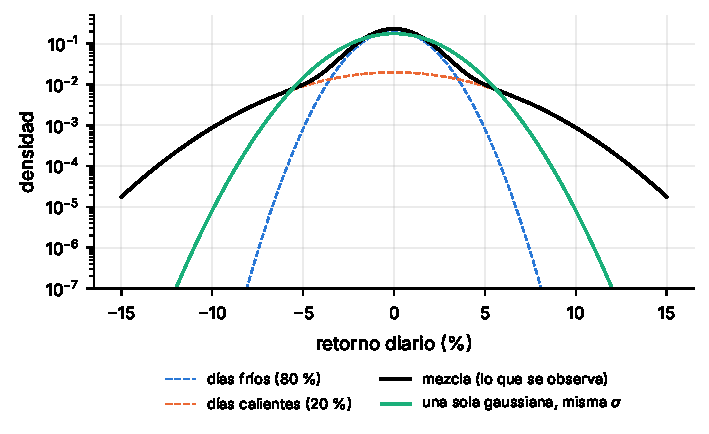
\includegraphics[width=0.72\textwidth]{fig2_mezcla.pdf}
\caption{Mezcla de un $80\%$ de días fríos ($\sigma=1.5\%$) y un $20\%$ de días calientes ($\sigma=4\%$),
frente a una sola gaussiana con la misma volatilidad total. Escala logarítmica.}
\label{fig:mezcla}
\end{figure}

Con una distribución continua de temperaturas el resultado es aún más llamativo. Si la inversa de la
varianza, $\beta=1/\sigma^2$ (el análogo de $1/k_BT$), sigue una distribución gamma, la mezcla de
gaussianas da exactamente una distribución $t$ de Student,
\begin{equation}
p(r)=\int_0^\infty\underbrace{\sqrt{\frac{\beta}{2\pi}}e^{-\beta r^2/2}}_{\text{gaussiana a temperatura }1/\beta}
f(\beta)\,\dd\beta\ \propto\ \left(1+\frac{r^2}{\nu s^2}\right)^{-(\nu+1)/2},
\end{equation}
cuyas colas decaen como una ley de potencias $|r|^{-(\nu+1)}$ y no como una exponencial de $-r^2$. Así se
obtienen colas gruesas a partir de física de equilibrio pura, a condición de dejar que la temperatura
fluctúe \cite{beck2003}.

\subsection{Un termómetro con memoria}

El termómetro de 20 días es tosco: trata igual un día de hace tres semanas que uno de ayer. Un modelo algo
mejor, y el más usado en finanzas, es el GARCH \cite{engle1982,bollerslev1986}. Escrito para la
temperatura $\sigma_t^2$ de cada día, dice
\begin{equation}
\sigma_t^2=\omega+\alpha\,r_{t-1}^2+\beta\,\sigma_{t-1}^2 .
\label{eq:garch}
\end{equation}
Se lee así: la temperatura de hoy es la suma de un nivel de fondo ($\omega$), del ``golpe'' de ayer
($r_{t-1}^2$: un día de movimiento grande calienta el mercado) y de la propia temperatura de ayer (la
inercia). Restando a ambos lados el nivel de equilibrio $\bar\sigma^2=\omega/(1-\alpha-\beta)$ se ve que
es una ley de relajación, como el enfriamiento de Newton, con golpes aleatorios:
\begin{equation}
\sigma_t^2-\bar\sigma^2=(\alpha+\beta)\left(\sigma_{t-1}^2-\bar\sigma^2\right)+\alpha\left(r_{t-1}^2-\sigma_{t-1}^2\right).
\end{equation}
El primer término hace que la temperatura vuelva a su valor medio; el segundo es un golpe de media cero.

Ajustando \eqref{eq:garch} a Google por máxima verosimilitud obtenemos $\alpha=0.057$ y $\beta=0.935$. La
\emph{persistencia} $\alpha+\beta=0.992$ es muy cercana a 1, y significa que la temperatura se relaja muy
despacio: una racha de agitación pierde la mitad de su exceso en $\ln(1/2)/\ln(0.992)\approx90$ días de
mercado, unos cuatro meses.

\subsection{Qué explica la temperatura y qué no}

Si la temperatura variable fuera la única causa de las colas gruesas, al dividir cada retorno por la
temperatura de su día, $z_t=r_t/\sigma_t$, deberíamos recuperar una gaussiana. \Cref{fig:normalizar}
muestra que mejora, pero no del todo: la curtosis baja de $7.6$ a $6.1$.

\begin{figure}[ht]
\centering
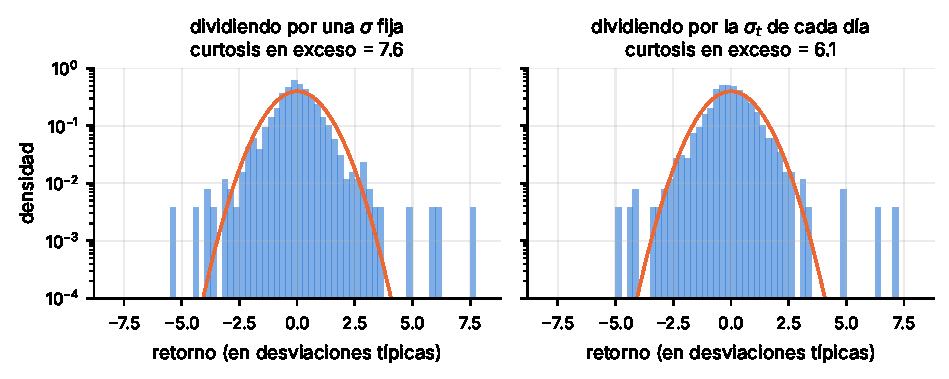
\includegraphics[width=0.95\textwidth]{fig2_normalizar.pdf}
\caption{Retornos de Google divididos por una volatilidad fija (izquierda) y por la temperatura de cada
día según el modelo GARCH (derecha), frente a la gaussiana.}
\label{fig:normalizar}
\end{figure}

Lo instructivo es mirar \emph{qué días} siguen siendo extremos. Estos son los seis mayores movimientos de
Google en el periodo, medidos con una volatilidad fija y con la temperatura del día:

\begin{table}[ht]
\centering\small
\caption{Los seis días más extremos de Google, en desviaciones típicas.}
\label{tab:seis}
\begin{tabular}{@{}lrrl@{}}
\toprule
Fecha & $\sigma$ fija & $\sigma_t$ del día & Qué pasó\\
\midrule
18-04-2008 & $+7.7$ & $+7.2$ & presentación de resultados trimestrales\\
22-10-2004 & $+6.0$ & $+4.9$ & presentación de resultados trimestrales\\
13-10-2008 & $+5.8$ & $+3.4$ & rebote general tras los rescates bancarios\\
29-09-2008 & $-5.3$ & $-4.4$ & caída general del mercado (crisis de 2008)\\
21-10-2005 & $+4.8$ & $+6.4$ & presentación de resultados trimestrales\\
18-07-2008 & $-4.4$ & $-4.9$ & presentación de resultados trimestrales\\
\bottomrule
\end{tabular}
\end{table}

Aparecen dos tipos de día. Los de la crisis de 2008 ocurrieron cuando el mercado ya estaba muy caliente,
y al medirlos con la temperatura del día dejan de ser tan extremos (de $5.8$ a $3.4$). Son exactamente lo
que describe la superestadística. Los otros cuatro son días en que Google presentó sus resultados
trimestrales (cuánto había ganado en los tres meses anteriores). Esa información llega de golpe, en una
fecha conocida pero con un contenido desconocido, y el precio salta. Ningún termómetro basado en el pasado
puede anticipar ese salto. En lenguaje físico, no son fluctuaciones térmicas sino \emph{fuerzas
impulsivas externas}: un golpe seco sobre la partícula, no el ruido del baño.

\subsection{La temperatura de mañana se puede predecir}

El agrupamiento de volatilidad tiene una consecuencia práctica importante. Hagamos un experimento honesto:
ajustamos el GARCH sólo con la primera mitad de los datos (hasta septiembre de 2006) y lo usamos para
predecir, cada día de la segunda mitad, la temperatura del día siguiente. Después ordenamos esos días en
cinco grupos, de los que el modelo predijo más fríos a los que predijo más calientes, y miramos qué pasó
de verdad (\cref{fig:prediccion}).

\begin{figure}[ht]
\centering
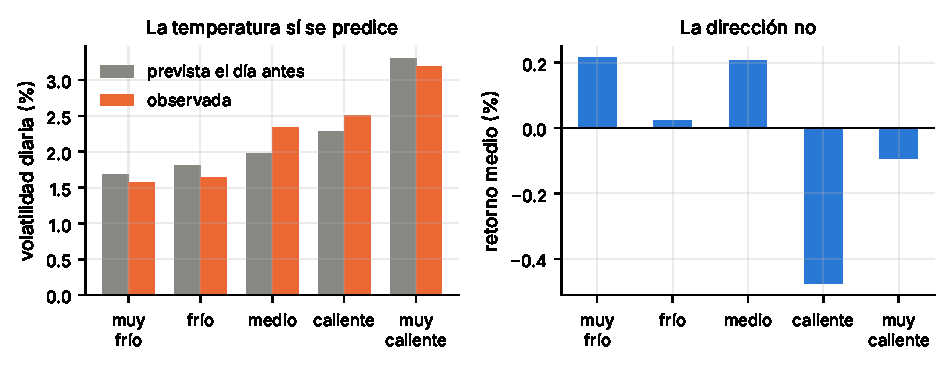
\includegraphics[width=0.95\textwidth]{fig2_prediccion.pdf}
\caption{Segunda mitad de los datos (septiembre de 2006 a octubre de 2008), nunca usada para ajustar el
modelo. Los días se reparten en cinco grupos según la temperatura prevista el día anterior. Izquierda:
volatilidad prevista y observada en cada grupo. Derecha: retorno medio en cada grupo.}
\label{fig:prediccion}
\end{figure}

La temperatura prevista va de $1.68\%$ a $3.31\%$ diario, y la observada, de $1.58\%$ a $3.20\%$: el modelo
acierta. En cambio, el retorno medio de cada grupo salta sin orden ($+0.22\%$, $+0.02\%$, $+0.21\%$,
$-0.48\%$, $-0.09\%$): saber que mañana será un día agitado no dice si será de subida o de bajada. Esta es
probablemente la lección más útil del documento: \emph{en un mercado, la dirección es casi impredecible,
pero el riesgo sí se puede predecir}. Un inversor puede usarlo como un termostato, invirtiendo menos cuando
el mercado se calienta y más cuando se enfría, para mantener su riesgo aproximadamente constante.

% =====================================================================
\section{Precios que vuelven: una partícula en un muelle}
\label{sec:muelle}
% =====================================================================

\subsection{El fenómeno económico}

El precio de una acción, como hemos visto, se comporta como un caminante libre: no hay ninguna fuerza que
lo devuelva a un sitio concreto. Pero hay magnitudes económicas que no pueden alejarse indefinidamente de
un valor ``normal''. El ejemplo típico es la diferencia de precio entre dos cosas muy parecidas: dos
compañías petroleras, Coca-Cola y Pepsi, o el mismo producto vendido en dos sitios. Si la diferencia se
hace demasiado grande, alguien comprará lo barato y venderá lo caro, y al hacerlo empujará los dos precios
el uno hacia el otro. Esa operación se llama \emph{arbitraje}, y actúa como una fuerza recuperadora. La
diferencia entre dos precios relacionados se suele llamar \emph{spread}.

\subsection{La física: Langevin con un muelle}

Imagina una partícula de polen atada a un muelle de constante $k$, sumergida en un líquido muy viscoso
(miel, por ejemplo). Sobre ella actúan tres fuerzas: la del muelle, $-k(x-\mu)$, que la devuelve a la
posición de equilibrio $\mu$; la fricción, $-\gamma\dot x$; y los choques térmicos de las moléculas,
$\eta(t)$. La ecuación de Langevin es
\begin{equation}
m\ddot x=-\gamma\dot x-k(x-\mu)+\eta(t) .
\end{equation}
En un líquido muy viscoso la inercia no importa (la partícula se para en cuanto deja de empujarla algo), y
podemos quitar el término $m\ddot x$. Dividiendo por $\gamma$ queda la ecuación de Ornstein--Uhlenbeck
\cite{uhlenbeck1930}:
\begin{equation}
\dd x=-\theta\,(x-\mu)\,\dd t+\sigma\,\dd W,\qquad \theta=\frac{k}{\gamma},\qquad
\sigma^2=\frac{2k_BT}{\gamma}.
\label{eq:ou}
\end{equation}
Aquí $\dd W$ es el ruido blanco (el incremento de un paseo aleatorio) y la última igualdad es la relación
de fluctuación--disipación de Einstein: el mismo líquido que frena la partícula es el que la agita, y por
eso la intensidad del ruido está ligada a la fricción y a la temperatura \cite{uam_me4,gardiner2009}.

Los dos parámetros tienen un significado claro:
\begin{itemize}
\item $\theta$ mide lo deprisa que el muelle devuelve la partícula. Un muelle rígido en un líquido poco
viscoso tiene $\theta$ grande.
\item $\sigma$ mide la intensidad del ruido térmico: cuánto la desordenan los choques.
\end{itemize}

\begin{table}[ht]
\centering\small
\caption{Diccionario de esta sección.}
\begin{tabular}{@{}ll@{}}
\toprule
Física & Mercado \\
\midrule
posición $x$ de la partícula & spread (diferencia entre dos precios)\\
posición de equilibrio $\mu$ & diferencia ``normal''\\
muelle $k$ & arbitraje: comprar lo barato y vender lo caro\\
fricción $\gamma$ & lo que tardan los operadores en reaccionar\\
choques térmicos & noticias y órdenes que afectan a uno y no al otro\\
vida media $\ln2/\theta$ & tiempo típico en que se corrige la mitad de un desvío\\
\bottomrule
\end{tabular}
\end{table}

\subsection{Cómo se mueve: relajación y vida media}

Tomando el valor medio de \eqref{eq:ou}, el ruido desaparece y queda $\dd\langle x\rangle/\dd t=-\theta(\langle
x\rangle-\mu)$, cuya solución es
\begin{equation}
\langle x(t)\rangle=\mu+(x_0-\mu)\,e^{-\theta t}.
\end{equation}
Un desvío inicial se corrige exponencialmente. El tiempo que tarda en reducirse a la mitad es la
\emph{vida media}, $t_{1/2}=\ln2/\theta$, la misma idea que en la desintegración radiactiva. Con
$\theta=0.05$ por día, $t_{1/2}=13.9$ días. \Cref{fig:pozo} muestra tres trayectorias simuladas que parten
de distintos desvíos: el muelle las devuelve hacia cero y, una vez allí, el ruido las mantiene
moviéndose alrededor.

\begin{figure}[ht]
\centering
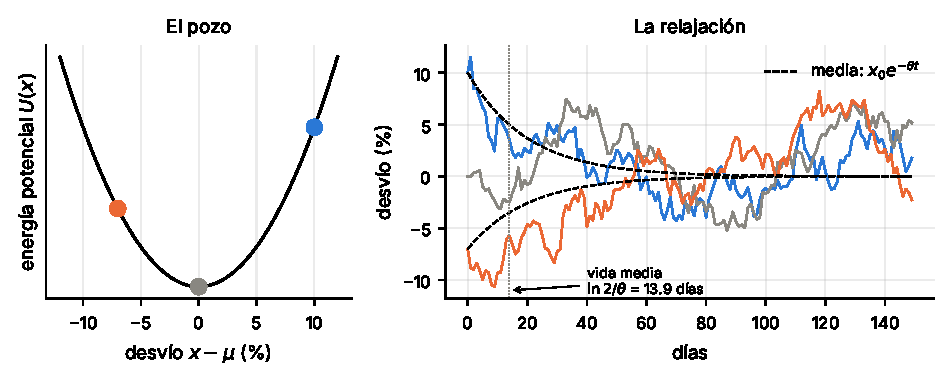
\includegraphics[width=0.95\textwidth]{fig3_pozo.pdf}
\caption{Izquierda: el pozo de potencial $U(x)=\tfrac12k(x-\mu)^2$ con tres posiciones iniciales. Derecha:
las tres trayectorias simuladas con $\theta=0.05$ por día y $\sigma=1\%$; las líneas discontinuas son la
relajación media $x_0e^{-\theta t}$.}
\label{fig:pozo}
\end{figure}

\subsection{El equilibrio es la distribución de Boltzmann}

Si esperamos mucho, la partícula olvida dónde empezó y su posición sigue una distribución estacionaria.
La forma más directa de encontrarla es la ecuación de Fokker--Planck asociada a \eqref{eq:ou}, que dice
cómo evoluciona la densidad de probabilidad:
\begin{equation}
\frac{\partial p}{\partial t}=\frac{\partial}{\partial x}\left[\theta(x-\mu)\,p\right]
+\frac{\sigma^2}{2}\frac{\partial^2p}{\partial x^2}.
\end{equation}
El primer término es el arrastre del muelle hacia el centro; el segundo, la difusión que lo aleja. En
equilibrio ambos se compensan y la solución es
\begin{equation}
p_{\text{eq}}(x)\propto\exp\left[-\frac{\theta(x-\mu)^2}{\sigma^2}\right]
=\exp\left[-\frac{U(x)}{k_BT}\right],
\end{equation}
donde en la segunda igualdad hemos usado $\theta=k/\gamma$ y $\sigma^2=2k_BT/\gamma$. Es la distribución de
Boltzmann de una partícula en un pozo armónico: una gaussiana de anchura $\sigma/\sqrt{2\theta}$. El muelle
y el ruido llegan a un compromiso, y la anchura de ese compromiso es la temperatura dividida por la
rigidez. Con los números del ejemplo, $1\%/\sqrt{0.1}=3.16\%$; en una simulación de 3000 días medimos
$3.10\%$ (\cref{fig:boltzmann}).

\begin{figure}[ht]
\centering
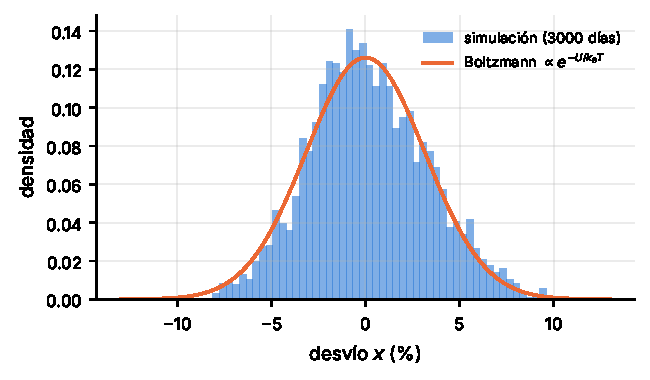
\includegraphics[width=0.62\textwidth]{fig3_boltzmann.pdf}
\caption{Histograma de una trayectoria simulada de 3000 días y la distribución de Boltzmann predicha.}
\label{fig:boltzmann}
\end{figure}

\subsection{Cómo se mide el muelle con datos}

Observando la partícula una vez al día, la solución exacta de \eqref{eq:ou} entre dos observaciones es
\begin{equation}
x_{t+1}-\mu=b\,(x_t-\mu)+\varepsilon_t,\qquad b=e^{-\theta}.
\end{equation}
Es decir: el desvío de mañana es una fracción $b$ del de hoy, más ruido. Así que basta con representar
$x_{t+1}$ frente a $x_t$ y ajustar una recta; su pendiente es $b$, y de ahí $\theta=-\ln b$. La lectura es
sencilla:
\begin{itemize}
\item $b$ pequeño: muelle fuerte, los desvíos se corrigen enseguida;
\item $b$ cerca de 1: muelle débil;
\item $b=1$: no hay muelle, es un paseo aleatorio.
\end{itemize}
En la simulación de 3000 días (con $\theta=0.05$, es decir, $b=0.951$) la recta da $b=0.949$, $\theta=0.052$
y una vida media de $13.2$ días, frente a los $13.9$ reales. El método funciona.

\subsection{Datos reales: ¿hay un muelle entre el Nasdaq y el S\&P~500?}

Los dos índices miden la bolsa estadounidense, uno con todas las grandes empresas y otro con sobre todo
tecnológicas, así que se mueven juntos. Ajustando $\ln(\text{Nasdaq})=1.34\,\ln(\text{S\&P})+c$ encontramos
que, cuando el S\&P~500 sube un $1\%$, el Nasdaq tiende a subir un $1.34\%$: las tecnológicas amplifican los
movimientos del mercado. Lo que sobra después de quitar esa relación es el spread (\cref{fig:spread}).

\begin{figure}[ht]
\centering
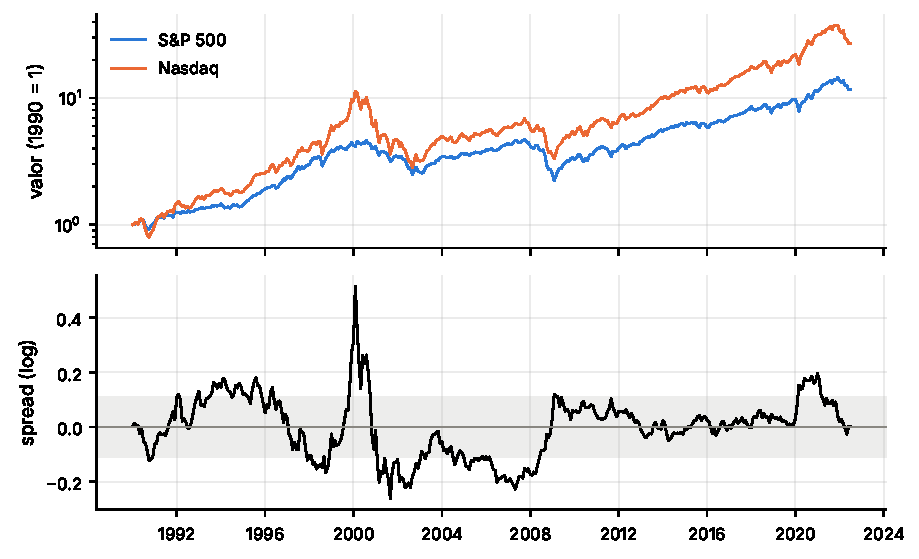
\includegraphics[width=0.95\textwidth]{fig3_spread.pdf}
\caption{Arriba: S\&P~500 y Nasdaq, 1990--2022 (valor relativo a 1990, escala logarítmica). Abajo: el spread
entre ambos; la banda gris marca una desviación típica.}
\label{fig:spread}
\end{figure}

Con la regresión de la sección anterior:
\begin{itemize}
\item el S\&P~500 por sí solo tiene $b=0.997$ al mes: una vida media de 216 meses, unos 18 años. A efectos
prácticos, ningún muelle. Es lo esperado para un precio (\cref{sec:paseo});
\item el spread tiene $b=0.956$: una vida media de 15 meses. Parece un muelle.
\end{itemize}

Pero aquí hay que tener cuidado, y es la parte más importante de esta sección. Hemos elegido el factor
$1.34$ con los mismos datos, buscando precisamente la combinación que mejor se ajusta; eso tiende a
fabricar un spread que parece volver a cero aunque no haya ningún muelle real. Para saber si el muelle
existe, hacemos un experimento de control: construimos 1000 parejas de paseos aleatorios
\emph{independientes}, con los mismos pasos mensuales que los dos índices pero barajados (sin ninguna
relación entre ellos), y les aplicamos exactamente el mismo procedimiento. En el $12\%$ de los casos sale un
$b$ tan pequeño como el real, o más. No podemos afirmar con seguridad que el muelle exista.

La razón se ve en la figura: el spread está dominado por un único episodio, el pico de 2000. Es la burbuja
de las empresas de internet, en la que el Nasdaq se multiplicó por cinco en pocos años y después perdió casi
el $80\%$. Con una vida media de 15 meses, treinta años de datos sólo contienen una veintena de
oscilaciones independientes, y una sola de ellas pesa demasiado. La burbuja, por cierto, no es un fenómeno
de muelles sino de imitación colectiva, y es el tema de la última sección.

La lección es útil también en la práctica. Existe una estrategia, el \emph{trading de pares}, que consiste
en comprar el activo relativamente barato y vender el caro cuando el spread se estira, esperando a que el
muelle lo devuelva. Sólo funciona si el muelle es real y no cambia con el tiempo, y comprobarlo exige
compararlo con lo que daría el azar.

% =====================================================================
\section{Imitación, burbujas y crashes: el modelo de Ising}
\label{sec:ising}
% =====================================================================

\subsection{El fenómeno económico}

Una \emph{burbuja} es una subida de precios mucho mayor de lo que justifican los beneficios de las
empresas: la gente compra porque el precio sube, y el precio sube porque la gente compra. Un \emph{crash}
es lo contrario: una caída brusca y colectiva, a menudo sin una noticia que la explique por sí sola. Los
dos fenómenos tienen algo en común: muchos inversores hacen a la vez lo mismo. Nadie decide en solitario
comprar en una burbuja o vender en un pánico; se mira lo que hacen los demás y se les imita. Es la misma
razón por la que elegimos el restaurante que está lleno \cite{kirman1993}.

\subsection{La física: espines que se alinean}

El modelo de Ising describe un imán como una red de espines $s_i=\pm1$. Cada espín prefiere apuntar como
sus vecinos (acoplamiento $J>0$) y como el campo magnético externo $h$. La energía de una configuración
es
\begin{equation}
E=-J\sum_{\langle ij\rangle}s_is_j-h\sum_is_i .
\end{equation}
A temperatura baja domina la energía y los espines se alinean: aparece una magnetización espontánea, el
imán. A temperatura alta domina la entropía (hay muchísimas más configuraciones desordenadas que
ordenadas) y la magnetización desaparece. Entre ambas fases hay una temperatura crítica $T_c$
\cite{uam_me3}.

\subsection{La traducción económica}

Cada espín es un inversor: $s_i=+1$ si compra y $s_i=-1$ si vende. La magnetización
\begin{equation}
m=\frac1N\sum_is_i
\end{equation}
es la fracción de compradores menos la fracción de vendedores, es decir, el \emph{exceso de demanda}.
Con $m=0.5$, compra el $75\%$ y vende el $25\%$. Como vimos en la introducción, el exceso de demanda es lo
que mueve el precio, así que en nuestras simulaciones lo modelamos de la forma más simple: cada día el
log-precio cambia en proporción a $m$, $\ln P_{t+1}=\ln P_t+\lambda m_t$.

\begin{table}[ht]
\centering\small
\caption{Diccionario de esta sección.}
\begin{tabular}{@{}ll@{}}
\toprule
Física & Mercado \\
\midrule
espín $s_i=\pm1$ & inversor que compra ($+1$) o vende ($-1$)\\
magnetización $m$ & exceso de demanda\\
acoplamiento $J$ & tendencia a imitar a los demás\\
campo externo $h$ & noticias que afectan a todos (buenas si $h>0$)\\
temperatura $T$ & diversidad de opiniones, decisiones independientes\\
fase ordenada ($T<T_c$) & consenso: burbuja o pánico\\
susceptibilidad $\chi$ & sensibilidad del mercado a las noticias\\
histéresis & el mercado no vuelve atrás por el mismo camino\\
\bottomrule
\end{tabular}
\end{table}

La temperatura merece un comentario. En el imán es agitación térmica; aquí representa todo lo que hace que
cada inversor decida por su cuenta: información propia, necesidades distintas (alguien vende porque
necesita el dinero, no porque espere una caída), opiniones diferentes. Un mercado ``caliente'' en este
sentido es un mercado con mucha diversidad, y eso lo hace estable. No hay que confundirlo con la
temperatura de la sección anterior, que medía la agitación de los precios. De hecho, veremos que son casi
opuestas: poca diversidad de opiniones produce precios muy agitados.

\Cref{fig:espines} muestra el modelo en una red cuadrada, en la que cada inversor sólo imita a sus cuatro
vecinos (por ejemplo, sus conocidos). Por debajo de $T_c$ casi todos compran; cerca de $T_c$ aparecen
grupos de todos los tamaños; por encima, cada uno va a lo suyo.

\begin{figure}[ht]
\centering
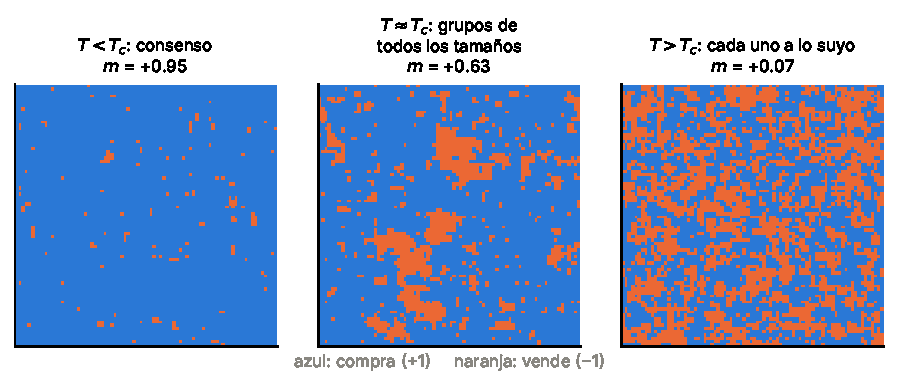
\includegraphics[width=0.95\textwidth]{fig4_espines.pdf}
\caption{Modelo de Ising en una red de $80\times80$ inversores, partiendo de que todos compran, a tres
temperaturas (en esta red $T_c=2.27\,J$).}
\label{fig:espines}
\end{figure}

\subsection{Campo medio: cada inversor mira la media}

En un mercado real nadie conoce sólo a cuatro vecinos: todos ven el precio, que resume lo que hacen todos.
Por eso usamos la versión de \emph{campo medio} del modelo, en la que cada inversor siente la opinión media
de los demás. El ``campo'' que nota el inversor $i$ es $Jm+h$: la presión de la mayoría más las noticias.
En equilibrio a temperatura $T$, la probabilidad de que compre es la de Boltzmann para un espín en ese
campo,
\begin{equation}
\Pr(s_i=+1)=\frac{e^{(Jm+h)/T}}{e^{(Jm+h)/T}+e^{-(Jm+h)/T}} ,
\end{equation}
y su valor medio es $\langle s_i\rangle=\tanh\left[(Jm+h)/T\right]$. Pero el valor medio de cada $s_i$ es, por
definición, $m$. Esto da la ecuación de autoconsistencia
\begin{equation}
m=\tanh\left(\frac{Jm+h}{T}\right).
\label{eq:weiss}
\end{equation}
Es una ecuación con $m$ a los dos lados: la opinión de cada uno depende de la de todos, y la de todos es la
suma de la de cada uno.

\Cref{fig:campo_medio} (izquierda) la resuelve gráficamente para $h=0$: los equilibrios son los cortes de
la recta $m$ con la curva $\tanh(Jm/T)$. La pendiente de la curva en el origen es $J/T$:
\begin{itemize}
\item si $T>J$, la curva es más plana que la recta y sólo se cortan en $m=0$: compradores y vendedores
equilibrados;
\item si $T<J$, la curva empieza más empinada y aparecen dos cortes más, $\pm m_0$: \emph{consenso sin
necesidad de noticias}.
\end{itemize}
La temperatura crítica es, por tanto, $T_c=J$. Por ejemplo, con $T=0.9\,J$ la solución es $m_0=0.53$: el
$76\%$ de los inversores compra (o vende) simplemente porque los demás lo hacen.

\begin{figure}[ht]
\centering
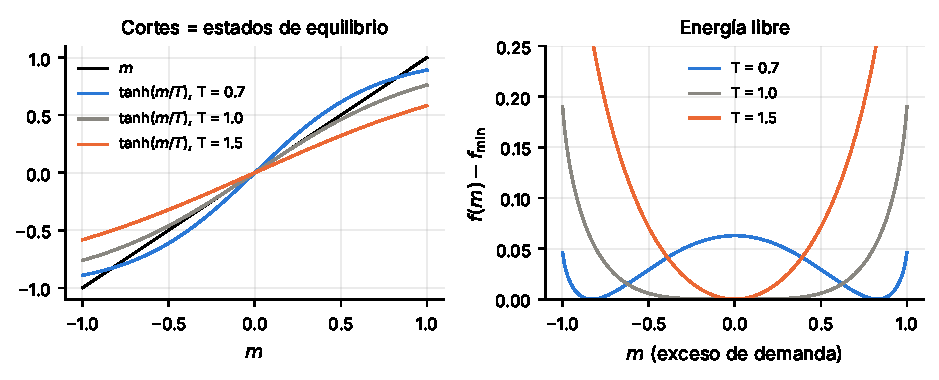
\includegraphics[width=0.95\textwidth]{fig4_campo_medio.pdf}
\caption{Izquierda: solución gráfica de $m=\tanh(m/T)$ con $J=1$; los equilibrios son los cortes con la
recta negra. Derecha: energía libre por inversor a las mismas tres temperaturas.}
\label{fig:campo_medio}
\end{figure}

\subsection{Energía frente a entropía}

La misma historia se ve en la energía libre por inversor (\cref{fig:campo_medio}, derecha):
\begin{equation}
f(m)=-\frac{J}{2}m^2-hm-T\,s(m),\qquad
s(m)=-\frac{1+m}{2}\ln\frac{1+m}{2}-\frac{1-m}{2}\ln\frac{1-m}{2}.
\end{equation}
El primer término premia el consenso. El último es la entropía, que cuenta de cuántas formas distintas se
puede conseguir un exceso de demanda $m$: hay muchísimas maneras de tener la mitad de compradores y una
sola de que compren todos. A temperatura alta gana la entropía y el mínimo está en $m=0$. Por debajo de
$T_c$ gana la imitación y aparecen dos valles, uno optimista y otro pesimista, separados por una barrera.

\subsection{Tres mercados simulados}

Para ver qué significa esto en precios, simulamos un mercado de 150 inversores que revisan su decisión al
azar, uno a uno, con la regla de Boltzmann anterior, y reciben cada día una pequeña noticia aleatoria
$h$. \Cref{fig:mercados} muestra el exceso de demanda y el precio a tres temperaturas.

\begin{figure}[ht]
\centering
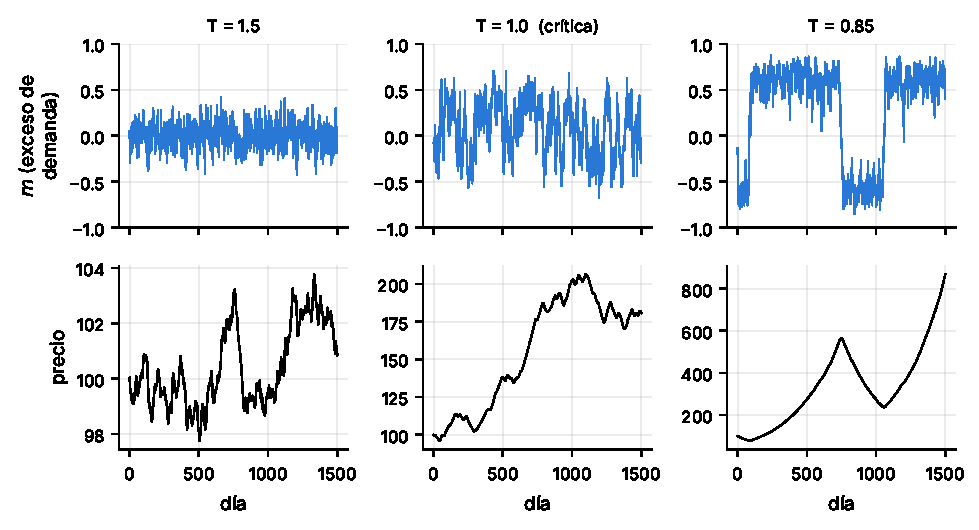
\includegraphics[width=0.95\textwidth]{fig4_mercados.pdf}
\caption{Mercado de Ising simulado durante 1500 días. Arriba: exceso de demanda $m$. Abajo: precio, que
cada día cambia en proporción a $m$. Izquierda: mucha diversidad de opiniones ($T=1.5\,J$). Centro: en el
punto crítico. Derecha: imitación dominante ($T=0.85\,J$).}
\label{fig:mercados}
\end{figure}

\begin{itemize}
\item Con $T=1.5\,J$, el exceso de demanda fluctúa alrededor de cero y el precio se parece a un paseo
aleatorio. Es el mercado de la \cref{sec:paseo}.
\item En el punto crítico, $T=J$, las fluctuaciones de $m$ se hacen grandes y lentas: el precio se mueve a
base de tendencias largas que se forman y se deshacen sin ninguna noticia importante. La autocorrelación de
$m$ de un día al siguiente pasa de $0.69$ a $0.94$.
\item Con $T=0.85\,J$, el mercado se queda atrapado durante cientos de días en uno de los dos valles: el
precio sube sin parar (una burbuja) o baja sin parar. De vez en cuando, una fluctuación lo hace cruzar la
barrera y el consenso se invierte bruscamente: un crash. En 1500 días hay 3 vuelcos.
\end{itemize}

\subsection{Susceptibilidad: noticias pequeñas, efectos grandes}

¿Cuánto cambia el exceso de demanda cuando llega una noticia? Eso es la susceptibilidad,
$\chi=\partial m/\partial h$. Derivando \eqref{eq:weiss} cerca de $m=0$ se obtiene, por encima de $T_c$,
\begin{equation}
\chi=\frac{1}{T-T_c},
\end{equation}
que diverge en el punto crítico (ley de Curie--Weiss). En la simulación no hace falta aplicar ninguna
noticia para medirla: por el teorema de fluctuación--disipación, la respuesta a un empujón es proporcional a
las fluctuaciones espontáneas, $\chi=N\,\mathrm{Var}(m)/T$. \Cref{fig:respuesta} (izquierda) muestra que la
simulación sigue la predicción: $\chi=1.03$ a $T=2J$ (teoría: 1) y $\chi=7.6$ a $T=1.1J$ (teoría: 10; la
diferencia se debe al tamaño finito del mercado).

La lectura económica es directa. En un mercado diverso, una noticia tiene un efecto proporcional a su
importancia. En un mercado cerca del punto crítico, donde todos se fijan mucho en lo que hacen los demás,
la misma noticia se amplifica de forma desproporcionada, porque cada inversor que reacciona arrastra a otros.

\begin{figure}[ht]
\centering
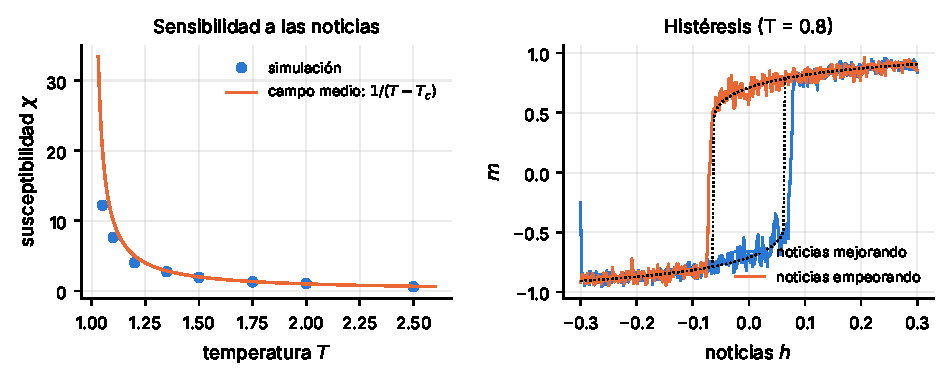
\includegraphics[width=0.95\textwidth]{fig4_respuesta.pdf}
\caption{Izquierda: susceptibilidad medida en la simulación y predicción de campo medio. Derecha:
exceso de demanda cuando las noticias mejoran poco a poco (azul) y después empeoran (naranja), a
$T=0.8\,J$. Las líneas de puntos son las dos ramas de la solución de campo medio.}
\label{fig:respuesta}
\end{figure}

\subsection{Histéresis: el crash como transición de primer orden}

El último experimento es el más revelador. A $T=0.8\,J$ empezamos con malas noticias ($h=-0.3$), que dejan
al mercado en el valle pesimista, y las vamos mejorando muy despacio hasta $h=+0.3$; después las empeoramos
igual de despacio (\cref{fig:respuesta}, derecha).

Cuando las noticias pasan a ser buenas ($h>0$), el mercado \emph{sigue siendo pesimista}: el valle
pesimista ya no es el más profundo, pero el mercado está dentro y no hay nada que lo saque. Sólo cuando
las noticias son claramente buenas, $h\approx0.07$, ese valle desaparece y el mercado salta de golpe al
optimismo. La teoría de campo medio predice que el valle desaparece en $h=0.062$; la simulación salta en
$h=0.074$. Al volver ocurre lo mismo al revés: el optimismo aguanta noticias malas hasta $h\approx-0.06$, y
entonces se desploma.

Es exactamente lo que pasa con el agua sobreenfriada, que puede seguir líquida por debajo de $0\,^\circ$C
hasta que de repente se congela entera. En términos de mercado, dice algo importante sobre los crashes:
\emph{no hace falta una noticia terrible para provocarlos}. Basta con que una serie de malas noticias
pequeñas, cada una de ellas inofensiva, lleve al sistema hasta el borde del valle. La última gota no es
mayor que las anteriores; simplemente es la que llega cuando el valle ya ha desaparecido. Y a la inversa,
el mercado puede tardar mucho en reaccionar a buenas noticias si viene de un pesimismo generalizado.

\subsection{Los límites del modelo}

Este Ising es deliberadamente sencillo: todos los inversores son iguales, todos ven a todos, y el precio
responde de forma lineal al exceso de demanda. Los modelos más realistas añaden inversores de varios tipos
(unos imitan, otros compran cuando el precio está barato y venden cuando está caro), y se ha mostrado que
reproducen tanto las colas gruesas como el agrupamiento de volatilidad de la \cref{sec:temp}
\cite{bornholdt2001}. También se ha intentado usar la idea del punto crítico para anticipar crashes
\cite{sornette2003}, con resultados discutidos. Lo que el modelo sencillo deja claro es el mecanismo:
imitación más diversidad decreciente igual a fluctuaciones grandes, lentas y, a veces, saltos bruscos.

% =====================================================================
\section{Conclusiones}
% =====================================================================

Las cuatro ideas encajan entre sí. El paseo aleatorio describe bien el día a día del precio: no tiene
memoria y su riesgo crece como la raíz del tiempo. Falla en los días extremos, y la temperatura explica
por qué: el mercado alterna épocas frías y calientes, y mezclar temperaturas produce colas gruesas. El
muelle describe las magnitudes que sí vuelven a su sitio, aunque demostrar que un muelle existe de verdad
exige compararlo con el azar. Y el modelo de Ising muestra cómo la imitación entre inversores puede
producir burbujas, crashes y una sensibilidad exagerada a las noticias.

\begin{table}[ht]
\centering\small
\caption{Resumen de lo que dicen los datos.}
\label{tab:resumen}
\begin{tabular}{@{}p{3.3cm}p{5.2cm}p{5.0cm}@{}}
\toprule
Idea & Qué predice & Qué hemos visto\\
\midrule
Paseo aleatorio & sin memoria; varianza $\propto t$; gaussiana & sí; sí (pendiente 1.10); no: colas gruesas\\
Temperatura & agrupamiento; colas por mezcla; temperatura predecible & sí ($C_{|r|}(1)=0.15$); en parte; sí, fuera de muestra\\
Muelle & desvíos que se corrigen con vida media fija & sí en simulación; en Nasdaq--S\&P no es concluyente ($p=0.12$)\\
Ising & consenso, susceptibilidad divergente, histéresis & reproducido en simulación\\
\bottomrule
\end{tabular}
\end{table}

Si hubiera que quedarse con una sola frase sería la de la \cref{sec:temp}: en un mercado, la dirección del
precio es casi impredecible, pero su temperatura sí se puede predecir. Toda la gestión del riesgo se
apoya en esa asimetría.

Hay tres continuaciones naturales de este trabajo. La primera, repetir los análisis con muchas acciones y
con datos de cada minuto, que multiplican por cientos el número de observaciones. La segunda, buscar
pares de activos con un muelle que supere la prueba del azar. La tercera, ajustar un modelo de Ising con
varios tipos de inversores a datos reales, para ver si su temperatura crítica dice algo sobre la llegada de
las crisis.

% =====================================================================
\appendix
\section{Cómo usar el código}
% =====================================================================

El repositorio tiene cinco archivos de Python. \texttt{comun.py} carga los datos y fija el estilo de las
figuras; los otros cuatro corresponden a las cuatro secciones y se ejecutan por separado:
\begin{verbatim}
pip install -r requirements.txt
python 01_paseo_aleatorio.py
python 02_temperatura.py
python 03_muelle.py
python 04_ising.py
\end{verbatim}
Cada uno guarda sus figuras en la carpeta \texttt{figuras/} e imprime en pantalla todos los números que
aparecen en este documento. Al principio de cada archivo hay un esquema con los tipos de datos que usa y
con los pasos que sigue, y cada bloque de código está comentado. Para analizar otra acción basta con
cambiar la función que carga los datos en \texttt{comun.py}.

\bibliographystyle{unsrt}
\bibliography{referencias}

\end{document}
